\documentclass[aps,twocolumn,superscriptaddress]{revtex4-1}
\usepackage{color}
\usepackage{graphicx}
\usepackage{epstopdf}
\epstopdfsetup{update}
\usepackage{amsmath}
\usepackage{amssymb}
\usepackage[colorlinks,linkcolor=blue,anchorcolor=blue,citecolor=blue,urlcolor=blue]{hyperref}

\newcommand{\bea}{\begin{eqnarray}}
\newcommand{\eea}{\end{eqnarray}}
\newcommand{\bF}{\mathbf{F}}
\newcommand{\ba}{\mathbf{a}}
\newcommand{\bA}{\mathbf{A}}
\newcommand{\bu}{\mathbf{u}}
\newcommand{\bg}{\mathbf{g}}
\newcommand{\bB}{\mathbf{B}}
\newcommand{\bd}{\mathbf{d}}
\newcommand{\be}{\mathbf{e}}
\newcommand{\bbm}{\mathbf{m}}
\newcommand{\bM}{\mathbf{M}}
\newcommand{\bv}{\mathbf{v}}
\newcommand{\bV}{\mathbf{V}}
\newcommand{\bp}{\mathbf{p}}
\newcommand{\bP}{\mathbf{P}}
\newcommand{\br}{\mathbf{r}}
\newcommand{\bx}{\mathbf{x}}
\newcommand{\bR}{\mathbf{R}}
\newcommand{\bN}{\mathbf{N}}
\newcommand{\bbell}{\boldsymbol{\ell}}
\newcommand{\bL}{\mathbf{L}}
\newcommand{\btau}{\boldsymbol{\tau}}
\newcommand{\bT}{\mathbf{T}}
\newcommand{\bi}{\mathbf{i}}
\newcommand{\bj}{\mathbf{j}}
\newcommand{\bk}{\mathbf{k}}
\newcommand{\bn}{\mathbf{n}}
\newcommand{\bomega}{\boldsymbol{\omega}}
\newcommand{\md}{\mathrm{d}}
\newcommand{\ie}{\textit{i.e.{ }}}
\newcommand{\eg}{\textit{e.g.{ }}}
\newcommand{\etc}{\textit{etc.{ }}}
\newcommand{\etal}{\textit{et al.{ }}}
\newcommand{\ddt}{\frac{\md}{\md t}}
\newcommand{\ddtt}{\frac{\md^2}{\md t^2}}
\newcommand{\ppt}{\frac{\partial}{\partial t}}
\newcommand{\pptt}{\frac{\partial^2}{\partial t^2}}
\newcommand{\me}{\mathrm{e}}


\begin{document}

\title{Multipartite entanglement among corner states in two dimensional second order topological insulators}
\author{Qiang Wang}
\affiliation{National Laboratory of Solid State Microstructures $\&$ School of Physics, Nanjing University, Nanjing, 210093, China}
\author{Da Wang}\email{dawang@nju.edu.cn}
\affiliation{National Laboratory of Solid State Microstructures $\&$ School of Physics, Nanjing University, Nanjing, 210093, China}
\author{Qiang-Hua Wang}\email{qhwang@nju.edu.cn}
\affiliation{National Laboratory of Solid State Microstructures $\&$ School of Physics, Nanjing University, Nanjing, 210093, China}
\affiliation{Collaborative Innovation Center of Advanced Microstructures, Nanjing University, Nanjing 210093, China}

\begin{abstract}
  In a $d$ dimensional topological insulator of order $d$, there are zero energy states on its 
  corners which have close relationship with its entanglement spectrum. 
  We first studied the effect of the subsystem shape on the single particle entanglement spectrum.
  We find out that only when the subsystem has a corner matching the lattice, exact zero energy states of the
  entangled Hamiltonian are obtained, corresponding to the zero energy mode on the physical corners.
  Next, we studied the fully entangled multi-partite state among these corner states which are coupled together
  by long range hybridizations caused by finite lattice size. We propose a scheme to calculate the quadripartite
  entanglement entropy on the square lattice, which is well described by a four-sites toy model 
  and thus can further identify such a second order topological insulator.
\end{abstract}
\maketitle
\section{introduction}
% close relation between entanglement and topological insulators
% high order topo, corner states, nested entanglement spectrum, corner contribution
% area law, topological entanglement entropy of long range entanglement, our scheme
Entanglement and topological states have close relationship, which is extensively studied in recent years.
\cite{Zeng2015,Laflorencie2017}
Generally speaking, a nontrivial structure of the entanglement spectra, \eg degeneracy of the many body one 
or gapless single particle one, always indicates a nontrivial topological state, and vice versa.
\cite{Ryu2006, Fidkowski2010}
The key point is the entanglement boundary in some sense mimics the physical boundary which further reflects the
topological property via the usual bulk boundary correspondence: a $d$ dimensional topological insulator 
has gapless states on its $d-1$ dimensional boundaries.


Very recently, a generalization of the topological insulator called high order topological insulator 
is theoretically predicted and observed in experiments.
\cite{}
Different from the conventional topological insulators, the gapless boundary states now exist 
on the $d-n$ dimensional boundaries for a $n$-th order topological insulator. 
The usual entanglement spectrum with cylindrical (smooth) bipartite scheme can not be directly applied 
to identify the high order topological insulators due to the missing of $d-1$ dimensional gapless boundary states.
However, a straightforward generalization can be conceived by choosing the subsystem 
with $d-n$ dimensional (non-smooth) entanglement boundary, in which case an additional 
contribution from the non-smooth corners \cite{Laflorencie2017} would lead to gapless entanglement spectra
and thus identify the high order topological insulators.
Such a scheme is proposed as nested entanglement spectra in literature. \cite{Schindler2017} 
In this work, we first focus on a special case with $n=d$ on a square lattice model 
to check the validity of this conjecture and examine the effect of the subsystem shape 
on the entanglement spectra. 
We find out that only when the corners of the subsystem match the lattice,
exact zero energy states of the entangled Hamiltonian exist 
which correspond to zero energy corner states. 

Next, on the other hand, in a real physical system with finite size, 
its zero energy boundary modes can be coupled together by long range hybridizations
and thus also contribute to the total entanglement entropy, which was proposed 
by one of the authors to identify the topological degeneracy induced by boundaries. \cite{Wang2015}
For the $d$-th order topological insulator with open boundary condition, 
the corner states are coupled together to form a fully multi-partite entangled state. 
We propose a scheme to extract the quadripartite entanglement entropy 
as a correction of the area law based on calculations on the whole lattice. 
We obtain a universal value of the quadripartite entanglement entropy 
which is well described by a toy model with only four sites
and thus directly identify the existence of these zero energy corner states. 


\section{model}

\begin{figure}
    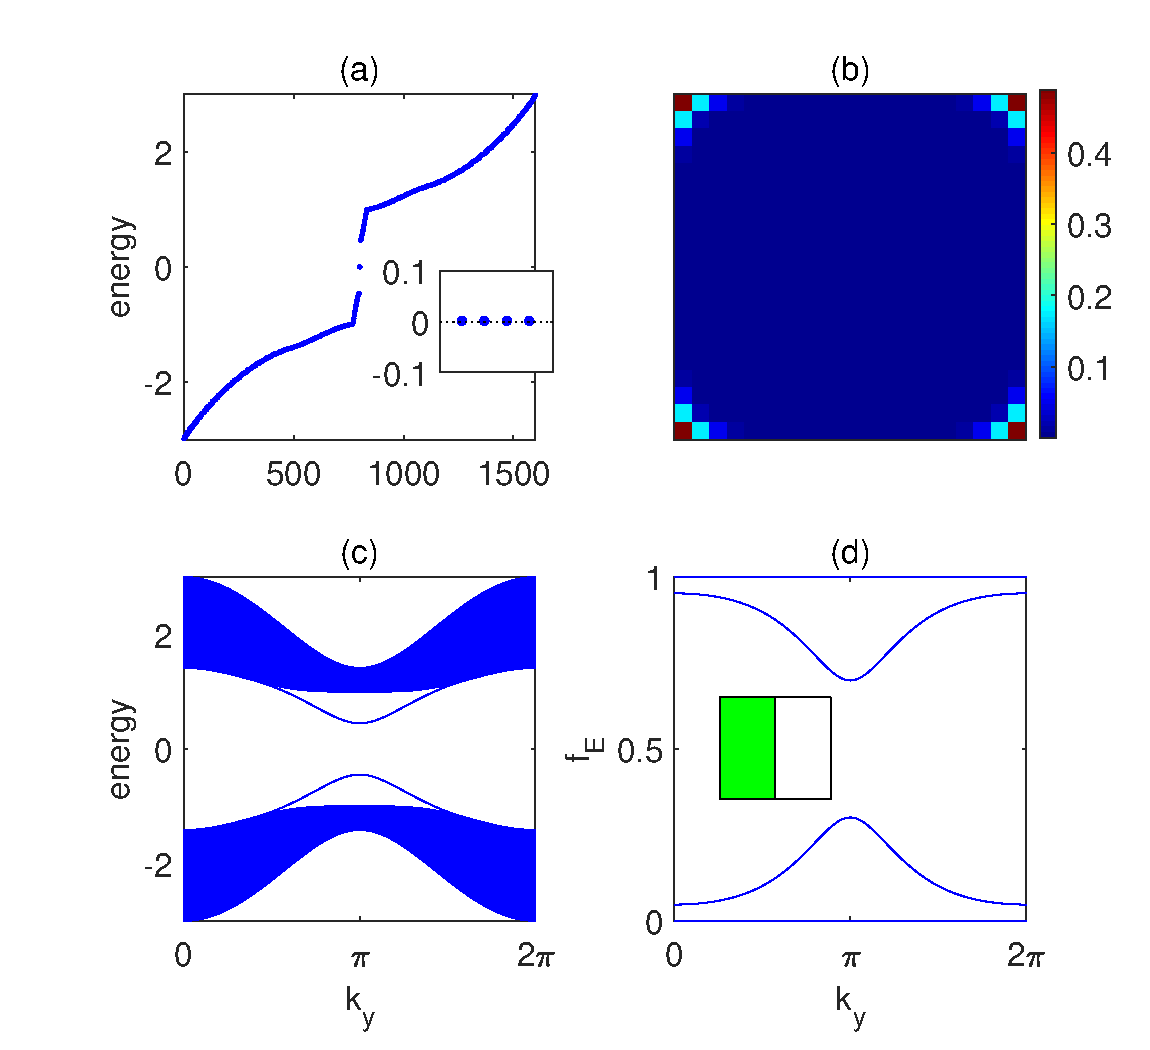
\includegraphics[width=0.5\textwidth]{model.eps}
    \caption{\label{fig:model} (a) Energy spectrum of a $20\times20$ lattice with open boundary condition.
    The inset shows the enlarged states near zero energy. (b) Local density of states of the zero modes.
    (c) Energy spectrum on a cylinder. (d) Entanglement occupation $f_E$ of the cylindrical bipartite
    scheme as shown in the inset where green region denotes the subsystem. }
\end{figure}

\section{corner contribution}

\begin{figure}
    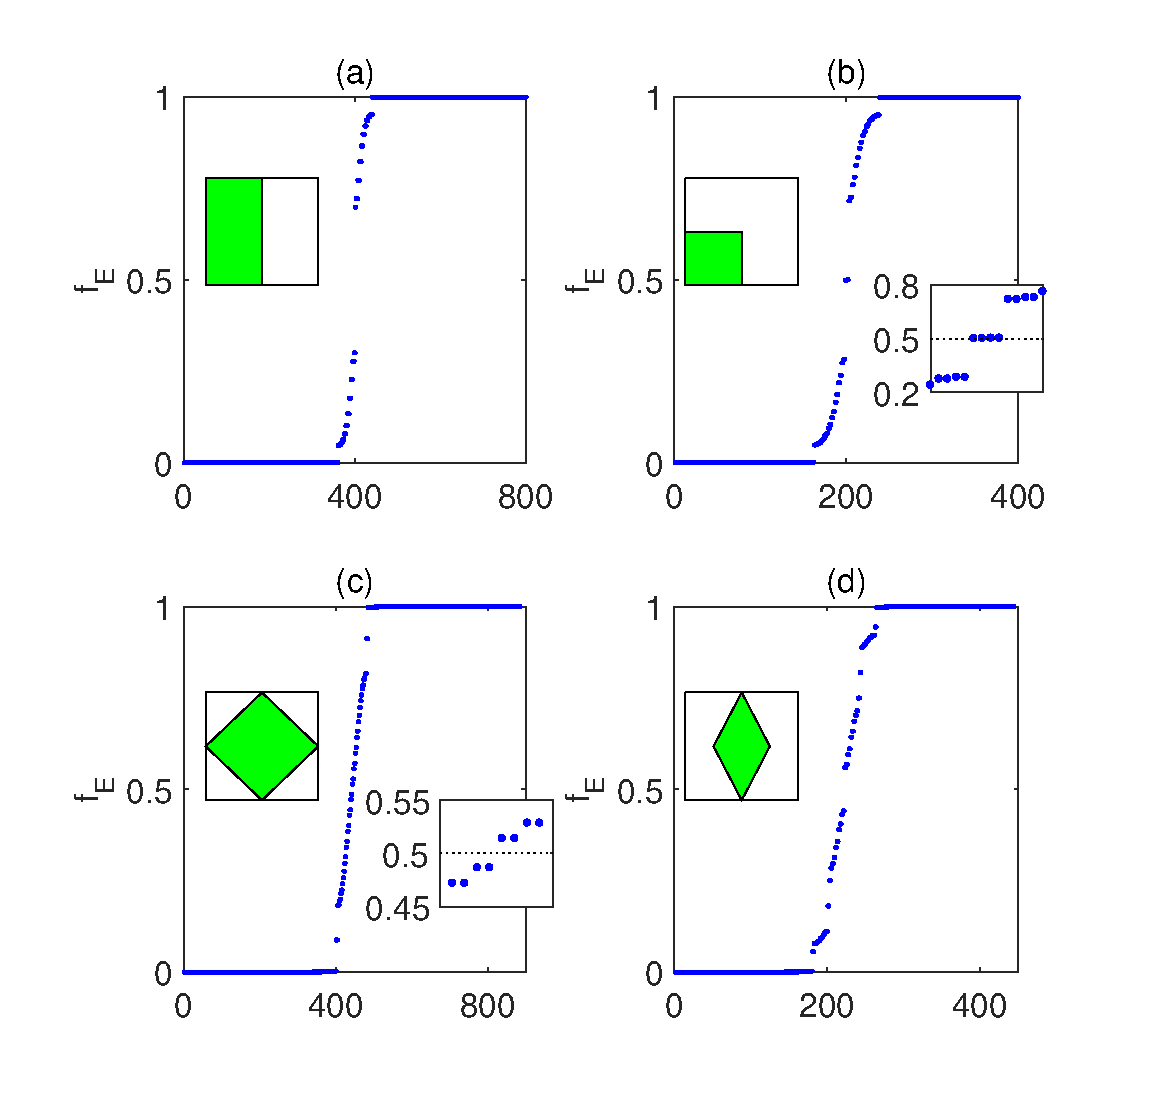
\includegraphics[width=0.5\textwidth]{subshape.eps}
    \caption{\label{fig:subshape} Entanglement occupation $f_E$ of different bipartite schemes from
    (a) to (d) as shown in their insets. In (b) and (c), the states near $f_E=0.5$ are also enlarged
    for clarity. }
\end{figure}

\section{quadripartite entanglement entropy}


\subsection{numerical result}

\begin{figure}
    \includegraphics[width=0.5\textwidth]{fourpartite.eps}
    \caption{\label{fig:fourpartite} Entanglement entropy in the case of open boundary condition. 
    We divide the whole lattice into four parts labeled by A, B, C and D, 
    respectively as shown in (a). Four red points denote four corner states.
    In (b) we plot $S_E(AB)$, $S_E(AD)$ and $S_E(AC)$ as functions of $L_y$ by fixing $L_x=20$.
    (c) shows $\Delta S_E=S_E(AB)+S_E(AD)-S_E(AC)$ as a function of $L_y$ for different $L_x$.
    Two dashed lines indicate two limits with $L_x=L_y$ and $L_x\ll L_y$(or $L_x\gg L_y$), respectively. 
    In large lattice size limit, a universal value $0.2797$ is obtained between the above two limits.
    In (d) a color plot of $\Delta S_E$ versus $L_x$ and $L_y$ is given. }
\end{figure}

\subsection{toy model}

In this section, we use a toy model including only four corner states to explain the numerically obtained universal
value of the quadripartite entanglement entropy. Soving the four-point tight binding model with only nearest hopping
together with a small flux (to break the degeneracy), its two occupied states are obtained
\begin{eqnarray}
  |\Psi_1\rangle&=&\frac12\left(|1\rangle-|2\rangle+|3\rangle-|4\rangle\right) \\
  |\Psi_2\rangle&=&\frac12\left(|1\rangle-i|2\rangle-|3\rangle+i|4\rangle\right) 
\end{eqnarray}
The total ground state is then given by $\Psi\rangle=|\Psi_1\rangle \times |\Psi_2\rangle$, which is a fully entangled
quadripartite state in space\footnote{In Fork space, it is a direct product state as a result of the non interacting
property}. Then the eigenvalues of the reduced correlation matrices can be easily solved out as
\begin{eqnarray}
  \lambda_{12}=\lambda_{14}=\left\{\frac{1}{2}+\frac{\sqrt{2}}{4},\frac{1}{2}-\frac{\sqrt{2}}{4}\right\}
\end{eqnarray}
and
\begin{eqnarray}
  \lambda_{13}=\left\{\frac{1}{2},\frac{1}{2}\right\}
\end{eqnarray}
which gives the quadripartite entanglement entropy
\begin{eqnarray}
  \Delta S= 4\ln2-\sqrt{2}\ln\frac{2+\sqrt{2}}{2-\sqrt{2}}=0.2797
\end{eqnarray}
The value is exactly the same as what we obtained in numerics by subtracting the result of $L_y\gg L_x$ 
from the square case with $L_y=L_x$ as $Lx\rightarrow\infty$. 
In contrast, in the toy model by setting $L_x\rightarrow\infty$, \ie cutting off the hoppings between sites $14$ and
$23$. Then, the gound state is a product state
\begin{eqnarray}
  |\Psi\rangle=|\Psi_{14}\rangle \times |\Psi_{23}\rangle
\end{eqnarray}
which gives $\Delta S=0$ clearly. Comparing with the numerical results on full lattice, it becomes clear that the
nonzero $\Delta S$ must come from the contribution from bulk states near the non-smooth corners of the entanglement 
boundary \cite{Laflorencie2016} similar to the nested entanglement spectrum\cite{Schindler2017}. 

\section{conclusion and discussion}

\section{acknowledgement}
This work is supported by NSFC (Nos. xxxx and yyyy).

\bibliography{ee2ti}
\end{document}
